\section{Cámaras como sensores}


\begin{frame}
\frametitle{Modelo de cámara}

\begin{block}{Definición - Cámara}
Una cámara es definida matemáticamente como una correspondencia entre el mundo 3D y una imagen 2D. Es decir, un mapeo entre puntos del mundo 3D $\point$ y puntos de la imagen $\imagePoint$:
\begin{equation}
\point=\begin{bmatrix}x\\
y\\
z
\end{bmatrix}\longmapsto
\imagePoint=\begin{bmatrix}u\\
v
\end{bmatrix}
\end{equation}
\end{block}

\end{frame}


\begin{frame}
\frametitle{Modelo de cámara pinhole}

\pnote{Llamamos rayo principal o eje principal de la cámara al rayo que se origina en el centro focal \cameraCenter y es perpendicular al plano de la imagen. El punto donde este rayo intersecta al plano de la imagen es denominado punto principal.}

\begin{block}{Cámara pinhole}
El punto de la imagen $\imagePoint=\begin{bmatrix}u & v\end{bmatrix}^{\top}$ es determinado como la intersección entre el \emph{plano de la imagen} y el rayo que une el punto del mundo 3D $\point=\begin{bmatrix}x & y & z\end{bmatrix}^{\top}$ con el \emph{centro focal} $\cameraCenter$ de la cámara.
\end{block}

\begin{figure}[!htb]
	\centering
	\subfloat[]{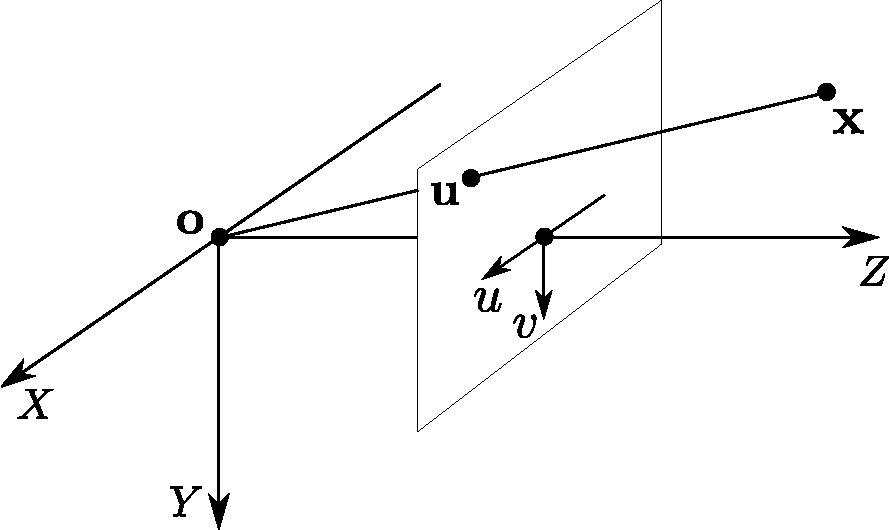
\includegraphics[width=0.5\columnwidth]{./cameras/pinhole_camera_model.pdf}}%
	\hfill
\end{figure}

\end{frame}


\begin{frame}
\frametitle{Modelo de cámara pinhole}

\begin{block}{Proyección central}
Asumiendo el centro focal en el origen de coordenadas y el plano de la imagen $Z=f$:

\begin{equation}
\begin{bmatrix}x\\
y\\
z
\end{bmatrix}\longmapsto\begin{bmatrix}fx/z\\
fy/z
\end{bmatrix}
\end{equation}

\end{block}

\begin{figure}[!htb]
	\centering
	\subfloat[]{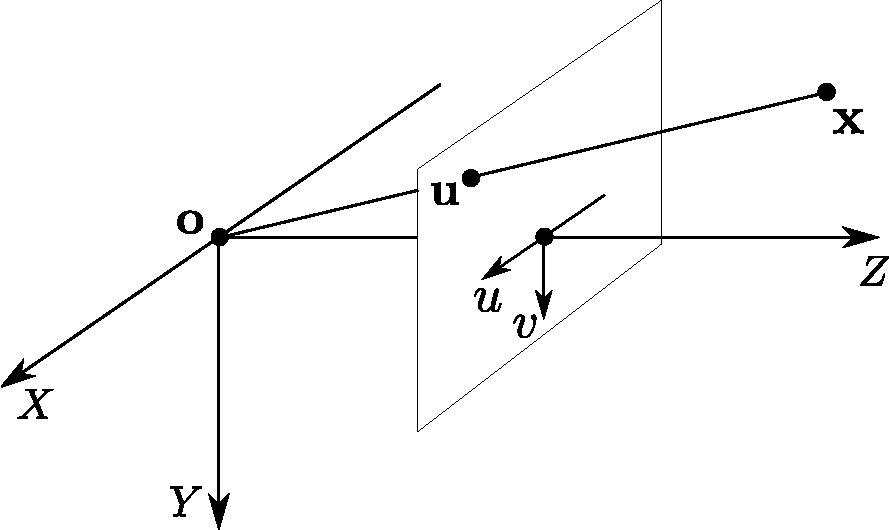
\includegraphics[width=0.5\columnwidth]{./cameras/pinhole_camera_model.pdf}}%
	\hfill
	\centering
	\subfloat[]{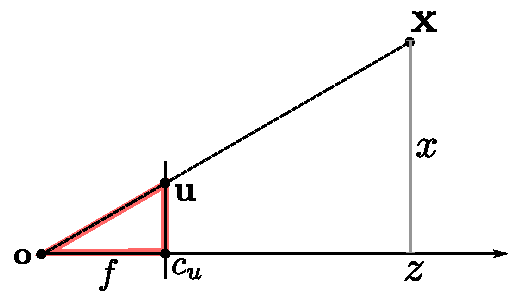
\includegraphics[width=0.5\columnwidth]{./cameras/pinhole_camera_model2.pdf}}%
	\hfill
\end{figure}

\end{frame}


\begin{frame}
\frametitle{Modelo de cámara pinhole}

Siendo $\begin{bmatrix}c_{u} & c_{v}\end{bmatrix}^{\top}$ la posición del punto principal.
\begin{equation}
\begin{bmatrix}x\\
y\\
z
\end{bmatrix}\longmapsto\begin{bmatrix}fx/z+c_{u}\\
fy/z+c_{v}
\end{bmatrix}
\end{equation}

En coordenadas homogéneas:

\begin{equation}
\begin{bmatrix}x\\
y\\
z\\
1
\end{bmatrix}\longmapsto\begin{bmatrix}fx+zc_{u}\\
fy+zc_{v}\\
z
\end{bmatrix}=\begin{bmatrix}f &  & c_{u} & 0\\
 & f & c_{v} & 0\\
 &  & 1 & 0
\end{bmatrix}\begin{bmatrix}x\\
y\\
z\\
1
\end{bmatrix}
\end{equation}

\begin{block}{Matriz de calibración intrínseca $\intrinsicMatrix$}
\begin{equation}
\intrinsicMatrix=\begin{bmatrix}f & 0 & c_{u}\\
0 & f & c_{v}\\
0 & 0 & 1
\end{bmatrix}
\end{equation}
\begin{equation}
\homo{\imagePoint}=\intrinsicMatrix\begin{bmatrix}\vec{{I}} & \vec{{0}}\end{bmatrix}\homo{\point}
\end{equation}
\end{block}

\end{frame}


\begin{frame}
\frametitle{Modelo de cámara pinhole}

Puntos expresados en referencia al sistema de coordenadas del \textit{mundo}. La cámara no se encuentra necesariamente ubicada en el centro de este.

\begin{figure}[!htb]
	\centering
	\subfloat[]{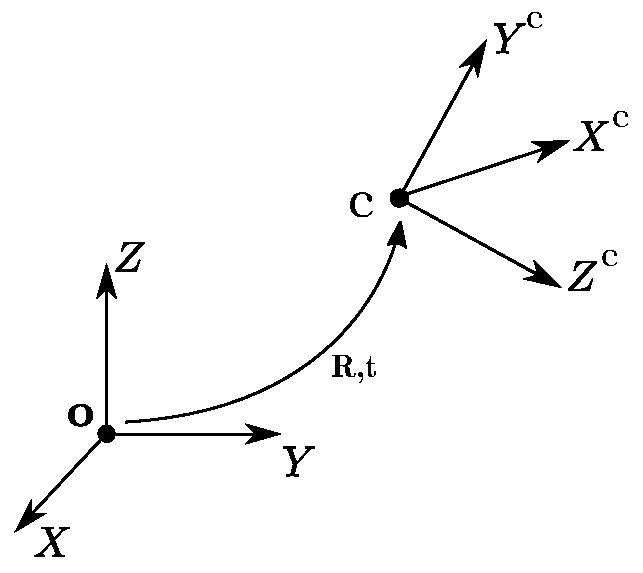
\includegraphics[width=0.4\columnwidth]{./cameras/camera_coord_system.pdf}}%
	\hfill
\end{figure}

\begin{block}{}
\begin{equation}
\homoCameraPoint=\begin{bmatrix}\rotation & \translation\\
0 & 1
\end{bmatrix}\begin{bmatrix}x\\
y\\
z\\
1
\end{bmatrix}=\seMatrix^{\mathrm{c}\mathrm{w}}\homoWorldPoint\;.
\end{equation}
\end{block}

\end{frame}


\begin{frame}
\frametitle{Modelo de cámara pinhole}

De esta manera, es posible proyectar cualquier punto 3D
$\homoWorldPoint$ en el sistema de coordenadas del mundo al correspondiente
punto $\homo{\imagePoint}$ en el plano de la imagen mediante:

\begin{block}{Matriz de proyección \textmd{$\projectionMatrix$}}
\begin{equation}
\projectionMatrix=\intrinsicMatrix\begin{bmatrix}\rotation & \translation\end{bmatrix}
\end{equation}
\begin{equation}
\homo{\imagePoint}=\projectionMatrix\homoWorldPoint
\end{equation}
\end{block}

\end{frame}